\section{Architecture}

We describe here the architecture of the control system that we have designed.
As specified in the assignment it is comprised of three separate controllers:
one for inputs from the console (named \texttt{Console}), one for
inputs from the sensors (named \texttt{Sensors}), and
one for outputs to the motors and the brakes (named \texttt{Output}).
Furthermore, we included another controller to orchestrate the correct functioning
of the others: one central processor (named \texttt{Processor}).
As general convention in the specification we use the prefix \texttt{r\_} to
indicate receive actions and \texttt{s\_} for send actions.

\begin{figure}[h]
    \centering
    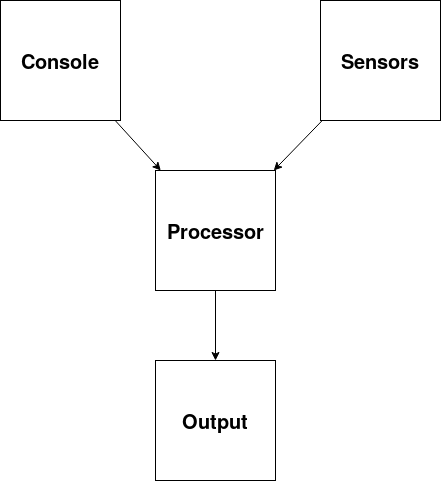
\includegraphics[width=0.6\textwidth]{img/system.png}
    \caption{Overall system architecture}
\end{figure}

\subsection{Console}

The console has 6 different buttons: \texttt{Up}, \texttt{Down},  \texttt{Stop},
\texttt{Reset},  \texttt{Undock} and \texttt{Resume}, as requested.
They can be both pressed and subsequently released or they can be tapped
(which is an atomic action).
When a button is pressed, released or tapped the corresponding send action
is sent to the processor, which will compute the input.

\begin{figure}[h]
    \centering
    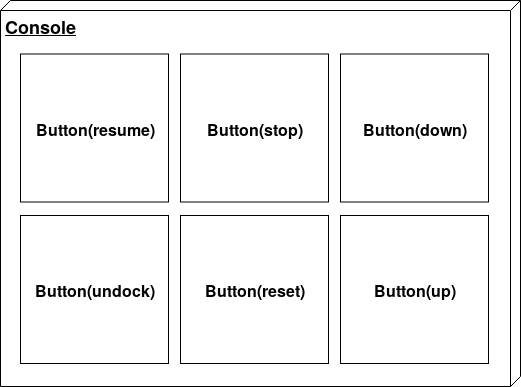
\includegraphics[width=0.7\textwidth]{img/console.png}
    \caption{Console controller}
\end{figure}

\subsection{Output}

The output controller accepts inputs from the processor through a secure channel
and simply executes the requests.
It is composed of five sub-components: the horizontal brake, the vertical brake,
the horizontal motor, the vertical motor and the undock controller.
The brakes can be released or applied, while the motors can move in two directions
(up/down or left/right) or they can be turned off.
The undock controller can be used to
undock the MPSP.
There is no "intelligence" in this output module, as all of the complexities to satisfy
the requirements are computed in the processor.
For example, if the processor sends the request to apply the vertical brake and
to move up at the same time, the motor will overheat.
Of course this won't happen, as the processor is designed to satisfy the requirements.

\begin{figure}[h]
    \centering
    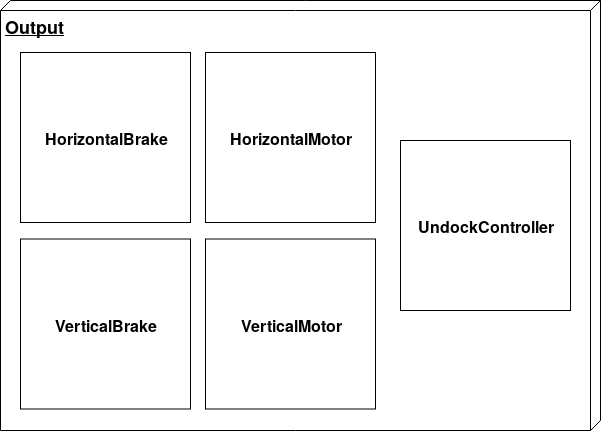
\includegraphics[width=0.7\textwidth]{img/output.png}
    \caption{Output controller}
\end{figure}

\subsection{Sensors}

The sensors accept input from the physical world and communicate them to the processor.
This module is composed of three sub-modules: the horizontal position sensors,
the vertical position sensors and the dock sensor.
The first can send the input rightmost or leftmost reached,
while the second can send uppermost, lowermost or standard height reached and
the last can send dock.
It is important to note that this module does not recognize if the movement
is done mechanically or manually, and for this reason the processor will have
to infer if a position message is due to motorized
movement or not.


\begin{figure}[h]
    \centering
    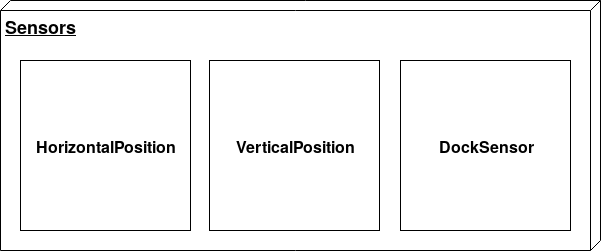
\includegraphics[width=0.7\textwidth]{img/sensors.png}
    \caption{Sensors controller}
\end{figure}

\subsection{Processor}

This controller keeps track of the current state of the system through one state variable.
It accepts inputs from the console and the sensors and, after processing them
it sends the proper output to the brakes, the motors or the undock controller.
It models the behavior requested in the assignment, and takes care of the
complexities related to satisfying the requirements (e.g. not applying the vertical
brake while the vertical motor is moving).

\subsection{Behavior}

The system is designed to work as described in the assignment, but sometimes
we had the freedom make our design decisions and not repeat the whole behavior of the system
as specified in the assignment.
In this section, we describe the complex behavior of the
MPSP and the autonomous decisions we made during the design of our system.

% TODO sei arrivato qui vecchio pazzo

\subsubsection{Initial state}

As it was not specified, we have decided that the initial state of the MPSP is:
\begin{itemize}
    \item Undocked
    \item Uncalibrated
    \item Vertical motor off
    \item Horizontal motor off
    \item Vertical brake applied
    \item Horizontal brake applied
    \item In normal mode
    \item At the lowermost position
\end{itemize}
This represents the scenario of a new MPSP delivered to the hospital
from the producer.

\subsubsection{Emergency mode}

The emergency mode can be activated only when the MPSP is docked.
If the emergency mode is triggered, we ensure that the horizontal
brake is not applied to allow medical staff to manually
remove locate the patient outside of the scanner. We thought that it is easier in the case of emergency, e.g. heart attack, to directly relocate the patients into the emergency section without removing them from the MPSP. For this reason, we decided that after triggering the emergency mode,
and after reaching the rightmost position,
the MPSP gets automatically undocked.
If the bed is already at the rightmost position, MPSP gets undocked. In case of the emergency mode, the bed reaches the rightmost position. Then the horizontal brakes is applied to prevent the patient from falling down.
Pressing or tapping the resume button puts the MPSP back to normal operating
mode.
This means that the MPSP can be docked, calibrated, etc.
While in emergency mode, no motorized movement can occur.

\subsubsection{Movement above the standard height}

As it is required that \emph{"While the MPSP is docked and calibrated,
the bed cannot be moved above the standard height"},
we decided that if the MPSP gets docked while calibrated and above the standard
height, if the button up is pressed or tapped, nothing happens.
Pressing the down button is the only actionb that lets the bed move.
It is possible to have the bed above the standard  height and docked
for example calibrating it, undocking it, while undocked pressing up
and then docking the MPSP.

\section{Implementation}

Although it was not requested, we want to point out some implementation details of the mCRL2 specification.

\subsection{Representation of the state}

While it was possible to store each state variable
(e.g. state of the brake, position etc) as a parameter of the processor
we decided to use one single variable of type \texttt{ProcessorState},
grouping all the variables in one single type. This has the advantage to produce more compact and clear mCRL2 specification.
To extract some variables from the state, we have implemented many utility
functions, for example \texttt{isAboveStandardHeight} or \texttt{isMovingUp}.

\subsection{Representation of the position}

The sensors can only inform the processor about certain points in the space (e.g. the lowermost position). The MPSP deduce the actual position also from the messages sent to the motors.
For example, if one action \lowermostReached\ occurred and then one \motorDown\ is sent to the motor, then the processor deduces that the position is somewhere between the uppermost and the lowermost position.

We don't need two separate variables for the vertical and the horizontal position, because if the MPSP has moved to the left, then it will be at the standard height.
For this reason we have eight possible values for the position:
\texttt{leftmost},
\texttt{horizontalBetween},
\texttt{lowermost},
\texttt{uppermost},
\texttt{verticalBetween},
\texttt{standardHeight},
\texttt{aboveStandardHeight} and
\texttt{belowStandardHeight}.
Also, we wanted to keep track if the MPSP is above or under the standard height when it is calibrated; therefore, we included the last two values.
The processor is able to determine whether it is correct to use either \texttt{aboveStandardHeight} or \texttt{verticalBetween} when moving up from the lowermost position, because it has the information if the bed is calibrated or not.

\subsection{Calibration}

We had trouble dealing with the fact that the MPSP could be calibrated at the uppermost position.
In fact, if the MPSP got subsequently undocked and the button reset was pressed at the standard height, there was no correct way to update the position in the state: the \texttt{uppermost} was not correct if the MPSP was calibrated under the uppermost position, and \texttt{horizontalbetween} was not correct if the MPSP was calibrated at the uppermost position.
We had the same problem for the lowermost position.
For this reason we decided to include in the calibration variable the fact that the MPSP can be calibrated at the uppermost or at the lowermost position.
The calibration is not a boolean value, but it can have four possible values:
\texttt{calibratedInBetween},
\texttt{calibratedUppermost},
\texttt{calibratedLowermost} and
\texttt{uncalibrated}.
In this way the processor is capable to correctly track the position of the MPSP.
